\documentclass[]{report}   % list options between brackets
\usepackage{amsmath}
\usepackage{amsfonts}
\usepackage{graphicx}
%\usepackage{}              % list packages between braces

% type user-defined commands here

\begin{document}

%%%%%%%%%%% Title page %%%%%%%%%%%

\title{Solid Object Visualisation Case Study}
%\subtitle{CS32310 Assignment Report}

\author{Hristoz Stefanov Stefanov}
\date{\today}

\maketitle





%%%%%%%%%%%% Abstract %%%%%%%%%%%%

\begin{abstract}

%> SEG instruction to authors <%
\begin{quotation}
	``Please pay particular attention to the preparation of your abstract; 
	use the material in this reference as a
	guide. Every manuscript other than a discussion must be accompanied by an informative abstract of no more than
	one paragraph (200 to 300 words). The abstract should be self-contained. No references, figures, tables, or
	equations are allowed in an abstract. Do not use new terminology in an abstract unless it is defined or is well
	known from prior publications. SEG discourages the use of commercial names or parenthetical statements. 
	The abstract must not simply list the topics covered in the paper but should (1) state the scope and principal
	objectives of the research, (2) describe the methods used, (3) summarize the results, and (4) state the principal
	conclusions. Do not refer to the paper itself in the abstract. For example, do not say, ``In this paper, we will
	discuss''

	The abstract must stand alone as a very short version of the paper rather than as a description of the contents.
	Remember that the abstract will be the most widely read portion of the paper. Various groups throughout the world
	publish abstracts of Geophysics papers. Readers and occasionally even reviewers may be influenced by the abstract
	to the point of final judgement before the body of the paper is read.''
\end{quotation}
%> SEG instruction to authors <%


Blah blah blah

\end{abstract}





%%%%%%%%% 1. Introduction %%%%%%%%

\chapter{Introduction}		% chapter 1


%> SEG instruction to authors <%
\begin{quotation}
	``The purpose of the introduction is to tell readers why they should want to read what follows the introduction.
	This section should provide sufficient background information to allow readers to understand the context and
	significance of the problem. This does not mean, however, that authors should use the introduction to rederive
	established results or to indulge in other needless repetition. The introduction should (1) present the nature
	and scope of the problem; (2) review the pertinent literature, within reason; (3) state the objectives; (4)
	describe the method of investigation; and (5) describe the principal results of the investigation.''
\end{quotation}
%> SEG instruction to authors <%


Blah blah blah





%%%%%%%%%%% 2. Methods %%%%%%%%%%%
\chapter{Methods}           % chapter 2

%> SEG instruction to authors <%
\begin{quotation}
	``The methodology employed in the work should be described in sufficient detail so that a competent geophysicist
	could duplicate the results. More detailed items (e.g., heavy mathematics) often are best placed in appendices.
	For complex mathematical articles, authors are strongly encouraged to include a table of symbols.''
\end{quotation}
%> SEG instruction to authors <%

Transformations are operations which can be carried out on geometric data. 
\[
	\mathbf{p\prime} = f(\mathbf{p})
\]



%----------- 2.1. Shift ----------
\section{Shift}

Shift (or translation) is one of the most basic linear transformations. Let \(\mathbf{p}\) be a point is space and \(\mathbf{t}\) be a vector describing the offset from that point. The new point \(\mathbf{p\prime}\) is then defined as:
\[
	\mathbf{p\prime} = \mathbf{p} + \mathbf{t}
\]

Note that a point has a position and no direction, while a vector has a direction and no position. Because of that operations between points and vectors (such as addition) are not defined, however a point \(\mathbf{p}\) can be expressed as a displacement \(\mathbf{t_p}\) from the origin of the coordinate system \(\mathbf{O}\). This property of points is often assumed and the displacement vector \(\mathbf{t_p}\) is what is implied instead. The same convention is used in this paper.


\subsection{Deriving a matrix}
In the case where \(\mathbf{p}, \mathbf{t} \in \mathbb{R}^3\) the above equation can also be expressed as a system of 3 equations (one for each axis).
\begin{align*}
	p\prime_x = p_x + t_x	\\
	p\prime_y = p_y + t_y	\\
	p\prime_z = p_z + t_z
\end{align*}

We can expand the equations slightly\dots
\begin{align*}
	p\prime_x = p_x 1+p_y 0+p_z 0+t_x	\\
	p\prime_y = p_x 0+p_y 1+p_z 0+t_y	\\
	p\prime_z = p_x 0+p_y 0+p_z 1+t_z
\end{align*}

\dots to make it obvious how we can derive the homogeneous 3D shift matrix.
\[
	\begin{bmatrix}
	p\prime_x \\
	p\prime_y \\
	p\prime_z \\
	1
	\end{bmatrix}
	=	
	\begin{bmatrix}
	1 & 0 & 0 & t_x \\
	0 &	1 & 0 & t_y \\
	0 & 0 & 1 &	t_z \\
	0 & 0 & 0 &	1
	\end{bmatrix}
	\begin{bmatrix}
		p_x \\
		p_y \\
		p_z \\
		1
	\end{bmatrix}
\]



%----------- 2.2. Scale ----------
\section{Scale}
Scale (or stretch) is another linear transformation which displaces a vector in certain proportion to its distance from the origin.

The simplest form of scale is:
\[ \mathbf{p\prime} = \alpha\mathbf{p} \]
Where \(\alpha\) is a scale factor. This function scales the original point \(\mathbf{p}\) homogeneously in all directions.



If we wanted to scale is a specific direction, let it be defined as the unit vector \(\mathbf{\hat{s}}\), we could do so by displacing the original point (in the direction \(\mathbf{\hat{s}}\)) by an amount equal to the projection of \(\mathbf{p}\) onto \(\mathbf{\hat{s}}\) scaled by a factor \(\alpha-1\) (see
\ref{fig:arb_axis_scale}).

\begin{figure}[htb]
\centering
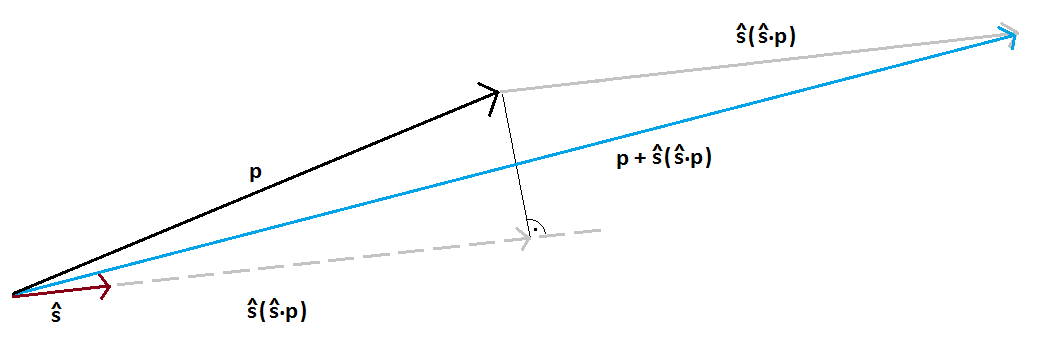
\includegraphics[width=0.9\textwidth]{arbitrary-axis-scale-diagram}
\caption{arbitrary axis scale}
\label{fig:arb_axis_scale}
\end{figure}

The resulting formula is this:
\[
	\mathbf{p\prime} = 
	\mathbf{p} + (\alpha - 1) \mathbf{\hat{s}}(\mathbf{\hat{s}}\cdot \mathbf{p})
\]

Let's consider the special case when \(\mathbf{p}\perp\mathbf{\hat{s}}\). In that case \(\mathbf{\hat{s}}\cdot \mathbf{p} = 0\), so we get the following equation:
\[
	\mathbf{p\prime} = 
	\mathbf{p} + (\alpha - 1) \mathbf{\hat{s}}0 = \mathbf{p} + \mathbf{0} = \mathbf{p}
\]
I.e. \(\mathbf{p}\) is unaffected by the scaling operation, which is what we would expect.

Another interesting case is when \(\mathbf{p}\parallel\mathbf{\hat{s}}\). In that case \(\mathbf{\hat{s}}\cdot \mathbf{p} = |\mathbf{p}|\), which is the maximal value the expression can acquire, which means scaling does the most shift.

Let \(\mathbf{\hat{s1}}\perp\mathbf{\hat{s2}}\) or \(\mathbf{\hat{s1}}\parallel\mathbf{\hat{s2}}\). If we do two subsequent scale transformations on vector \(\mathbf{p}\) along each of the two axis the resulting point \(\mathbf{p\prime}\) the same regardless of the order of the operations. If none of the two conditions holds true then \(\mathbf{p\prime}\) will be more affected by the direction vector to be used for the first scaling operation. Given this, let \(\mathbf{\hat{x}}\perp\mathbf{\hat{y}}\perp\mathbf{\hat{z}}\); \(\mathbf{\hat{x}},\mathbf{\hat{y}},\mathbf{\hat{z}},\mathbf{\hat{p}} \in \mathbb{R}^3\) and \(\alpha,\beta\) and \(\gamma\) be scale actors along each vector respectively. We can combine 3 subsequent scaling operations in each direction into a single formula:
\[
	\mathbf{p\prime} = 
	\alpha \mathbf{\hat{x}}( \mathbf{p} \cdot \mathbf{\hat{x}}) +
	\beta \mathbf{\hat{y}}( \mathbf{p} \cdot \mathbf{\hat{y}}) +
	\gamma \mathbf{\hat{z}}( \mathbf{p} \cdot \mathbf{\hat{z}})
\]


\subsection{Deriving a matrix}

In the case where \(\mathbf{p},\mathbf{\hat{s}} \in \mathbb{R}^3\) we can decompose the arbitrary axis equation in the following system of 3 equations:
\begin{align*}
	p\prime_x = p_x + (\alpha - 1)s_x(s_x p_x +	s_y p_y + s_z p_z)	\\
	p\prime_y = p_y + (\alpha - 1)s_y(s_x p_x +	s_y p_y + s_z p_z)	\\
	p\prime_z = p_z + (\alpha - 1)s_z(s_x p_x +	s_y p_y + s_z p_z)
\end{align*}

We can rearrange each so that we have only one occurrence of \(p_x, p_y, p_z, p\prime_x, p\prime_y\) and \(p\prime_z\). And we get the following:
\begin{align*}
	p\prime_x = (1 + (\alpha - 1)s_x^2)p_x + (\alpha - 1)s_x s_y p_y + (\alpha - 1)s_x s_z p_z	\\
	p\prime_y = (\alpha - 1)s_y s_x p_x + (1 + (\alpha - 1)s_y^2)p_y + (\alpha - 1)s_y s_z p_z	\\
	p\prime_z = (\alpha - 1)s_z s_x p_x + (\alpha - 1)s_z s_y p_y + (1 + (\alpha - 1)s_z^2)p_z
\end{align*}

Extracting a homogeneous 3D matrix from the above system of equations is easy.
\[
	\begin{bmatrix}
	p\prime_x \\
	p\prime_y \\
	p\prime_z \\
	1
	\end{bmatrix}
	=	
	\begin{bmatrix}
	1 + (\alpha - 1)s_x^2 & (\alpha - 1)s_x s_y & (\alpha - 1)s_x s_z &  0  \\
	(\alpha - 1)s_x s_y & 1 + (\alpha - 1)s_y^2 & (\alpha - 1)s_y s_z &  0  \\
	(\alpha - 1)s_x s_z & (\alpha - 1)s_y s_z  & 1 + (\alpha - 1)s_z^2 & 0  \\
	0 & 0 & 0 &	1
	\end{bmatrix}
	\begin{bmatrix}
		p_x \\
		p_y \\
		p_z \\
		1
	\end{bmatrix}
\]


Now, let \(\mathbf{\hat{x}} =(1,0,0); \mathbf{\hat{y}} =(0,1,0); \mathbf{\hat{z}} =(0,0,1)\) and \(\alpha,\beta\) and \(\gamma\) be scale factors in each direction respectively. If we replaced \(\mathbf{\hat{s}}\) in the above matrix, with each and multiplied the 3 resulting matrices (after simplifying) we would get:
\[
	\mathbf{A} =
	\begin{bmatrix}
		\alpha & 0 & 0 & 0 \\
		0 &	1 & 0 & 0 \\
		0 & 0 & 1 &	0 \\
		0 & 0 & 0 &	1
	\end{bmatrix}
	\begin{bmatrix}
		1 & 0 & 0 & 0 \\
		0 &	\beta & 0 & 0 \\
		0 & 0 & 1 &	0 \\
		0 & 0 & 0 &	1
	\end{bmatrix}
	\begin{bmatrix}
		1 & 0 & 0 & 0 \\
		0 &	1 & 0 & 0 \\
		0 & 0 & \gamma &	0 \\
		0 & 0 & 0 &	1
	\end{bmatrix}
	=
	\begin{bmatrix}
		\alpha & 0 & 0 & 0 \\
		0 &	\beta & 0 & 0 \\
		0 & 0 & \gamma &	0 \\
		0 & 0 & 0 &	1
	\end{bmatrix}	
\]
Note that the order of the multiplication does not matter as \(\mathbf{\hat{x}}, \mathbf{\hat{y}}\) and \(\mathbf{\hat{z}}\) are mutually perpendicular.
 


%---------- 2.3. Rotate ----------
\section{Rotate}

Blah blah blah


%---------- 2.4. Reflect ---------
\section{Reflect}

Reflection is a linear operation, where a point \(\mathbf{p}\) is translated twice its distance to a reflector plane in a direction opposite to the normal vector of that plane. Consider the diagram \ref{fig:reflect}:

\begin{figure}[htb]
\centering
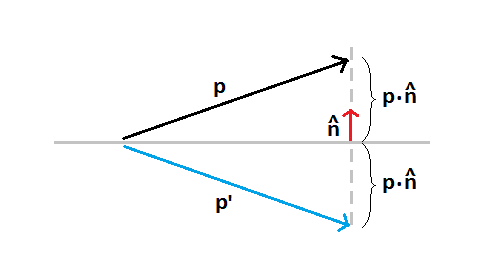
\includegraphics[width=0.9\textwidth]{reflection-diagram}
\caption{reflection}
\label{fig:reflect}
\end{figure}

The formula then becomes obvious:
\[
	\mathbf{p\prime} = 
	\mathbf{p} - 2\mathbf{\hat{n}}(\mathbf{\hat{n}} \cdot \mathbf{p})
\]

If \(\mathbf{p}\) lies on the plane then \(\mathbf{\hat{n}} \cdot \mathbf{p} = 0\), so we get that \(\mathbf{p\prime} = \mathbf{p}\), which shouldn't be surprising. 

Another thing we might want to consider is when \(\mathbf{p}\) is behind the plane. In that case \(\mathbf{\hat{n}} \cdot \mathbf{p} < 0\) which means we'll be going in the direction of the plane normal (rather than it's opposite), so \(\mathbf{p\prime}\) will be in front of the plane. This also means that if we applied the same reflection transformation to a point twice (or any even number of times) we would get the same point.


\subsection{Deriving a matrix}
Deriving a 3D matrix is again quite easy. We first decompose the equation:
\begin{align*}
	p\prime_x = p_x - 2n_x(n_x p_x + n_y p_y + n_z p_z)		\\
	p\prime_y = p_y - 2n_y(n_x p_x + n_y p_y + n_z p_z)		\\
	p\prime_z = p_z - 2n_z(n_x p_x + n_y p_y + n_z p_z)		\\
\end{align*}

Then rearrange so that we only have one occurance of \(p_x, p_y, p_z, p\prime_x, p\prime_y\) and \(p\prime_z\)and we arrive at:

\begin{align*}
	p\prime_x &= (1 - 2n_x^2)p_x -2n_x n_y p_y -2n_x n_z p_z	\\
	p\prime_y &= -2n_x n_y p_x + (1 - 2n_y^2)p_y -2n_y n_z p_z	\\
	p\prime_z &= -2n_x n_z p_x -2n_y n_z p_y + (1 - 2n_z^2)p_z	\\
\end{align*}

Which maps perfectly into a 3x3 matrix:

\[
	\begin{bmatrix}
	p\prime_x \\
	p\prime_y \\
	p\prime_z \\
	1
	\end{bmatrix}
	=	
	\begin{bmatrix}
		1 - 2n_x^2	&	-2n_x n_y	&	-2n_x n_z	&	0 \\
		-2n_x n_y	&	1 - 2n_y^2	& 	-2n_y n_z	&	0 \\
		-2n_x n_z	&	-2n_y n_z	&	1 - 2n_z^2	&	0 \\
		0 			&		0 		& 		0 		&	1
	\end{bmatrix}
	\begin{bmatrix}
		p_x \\
		p_y \\
		p_z \\
		1
	\end{bmatrix}
\]


%------ 2.5. Parallel Proj. ------
\section{Parallel Projection}
Parrallel projection is a linear transformation which maps a point in a 3D scene onto a projection plane, where the distance of an object from the projection plane does not affect its appearance.

We could achieve the effect of parallel projection similarly to the reflection transformation discussed earlier.
The only difference would be instead of going twice the distance in the direction opposite to the surface normal,
we go once. In other words using this formula:
\[
	\mathbf{p\prime} = 
	\mathbf{p} - \mathbf{\hat{n}}(\mathbf{\hat{n}} \cdot \mathbf{p})
\]

This would effectively translate \(\mathbf{p}\) onto the surface defined by the normal \(\mathbf{\hat{n}}\), but lets consider a slightly more complex situation. The above equation would transfer the point \(\mathbf{p}\) directly onto the surface in the directon of the normal \(\mathbf{\hat{n}}\) and is a special case of parallel projection called orthographic projection, however that might not be sufficient, if we wanted to view.... <MESS, correct!>

%Parallel projection
%p' = p -  (n.p)/(n.c) * c

%----- 2.6. Perspective Proj. ----
\section{Perspective Projection}

Blah blah blah





%%%%%%%%%%% 3. Results %%%%%%%%%%%
\chapter{Results}           % chapter 3

%> SEG instruction to authors <%
\begin{quotation}
	``The results section contains applications of the methodology described above. The results of experiments
	(either physical or computational) are data and can be presented as tables or figures and analyses. Whenever
	possible, include at least one example of recorded data to illustrate the technology or concept being proposed.
	Case-history results are usually geologic interpretations.

	Selective presentation of results is important. Redundancy should be avoided, and results of minor variations on
	the principal experiment should be summarized rather than included. Details appearing in figure captions and
	table heads should not be restated in the text. In a well-written paper, the results section is often the
	shortest.''
\end{quotation}
%> SEG instruction to authors <%


Blah blah blah





%%%%%%%%%% 4. Conclusion %%%%%%%%%
\chapter{Conclusion}		% chapter 4

%> SEG instruction to authors <%
\begin{quotation}
	``The conclusion section should include (1) principles, relationships, and generalizations inferred from the
	results (but not a repetition of the results); (2) any exceptions to or problems with those principles,
	relationships, and generalizations, as indicated by the results; (3) agreements or disagreements with previously
	published work; (4) theoretical implications and possible practical applications of the work; and (5) conclusions
	drawn (especially regarding significance). In particular, with reference to item (1) above, a conclusion that
	only summarizes the results is not acceptable.''
\end{quotation}
%> SEG instruction to authors <%


Blah blah blah






%%%%%%%%%% Bibliography %%%%%%%%%%
\begin{thebibliography}{9}
  % type bibliography here
\end{thebibliography}





\end{document}